
\section{Testing}
\label{s:Testing}
Testing is a crucial aspect in Software Engineering, so much important that many
advocate the use of Test-Driven Development, especially in the Agile world.
Test-Driven Development is a process of having tests before anything else,
developing them before the code of the software has been written yet, and using
such tests to verify the correct behaviour of the business logic. It is a very
important methodology, but it was tough to work with it during this project
because of the highly nested data structure that the abstract syntax tree would
return on the manipulation. For this reason, tests have been written later to
ensure vast use-cases and find bugs using large schemas as the starting point
for a mock generation. This project uses Snapshot testing to guarantee
consistent behaviour in the output of generated objects. That can be very useful
because of changes to the logic that can cause everything to break. Such tests
would instantly recognise that and fail.

The test files sit in the \texttt{src/\_\_tests\_\_folder} and test the
behaviour of two main functions, which are the core of the whole application:
formatItem and formatSchema. A screenshot of one of a test below:

\begin{figure}[H]
  \centering
  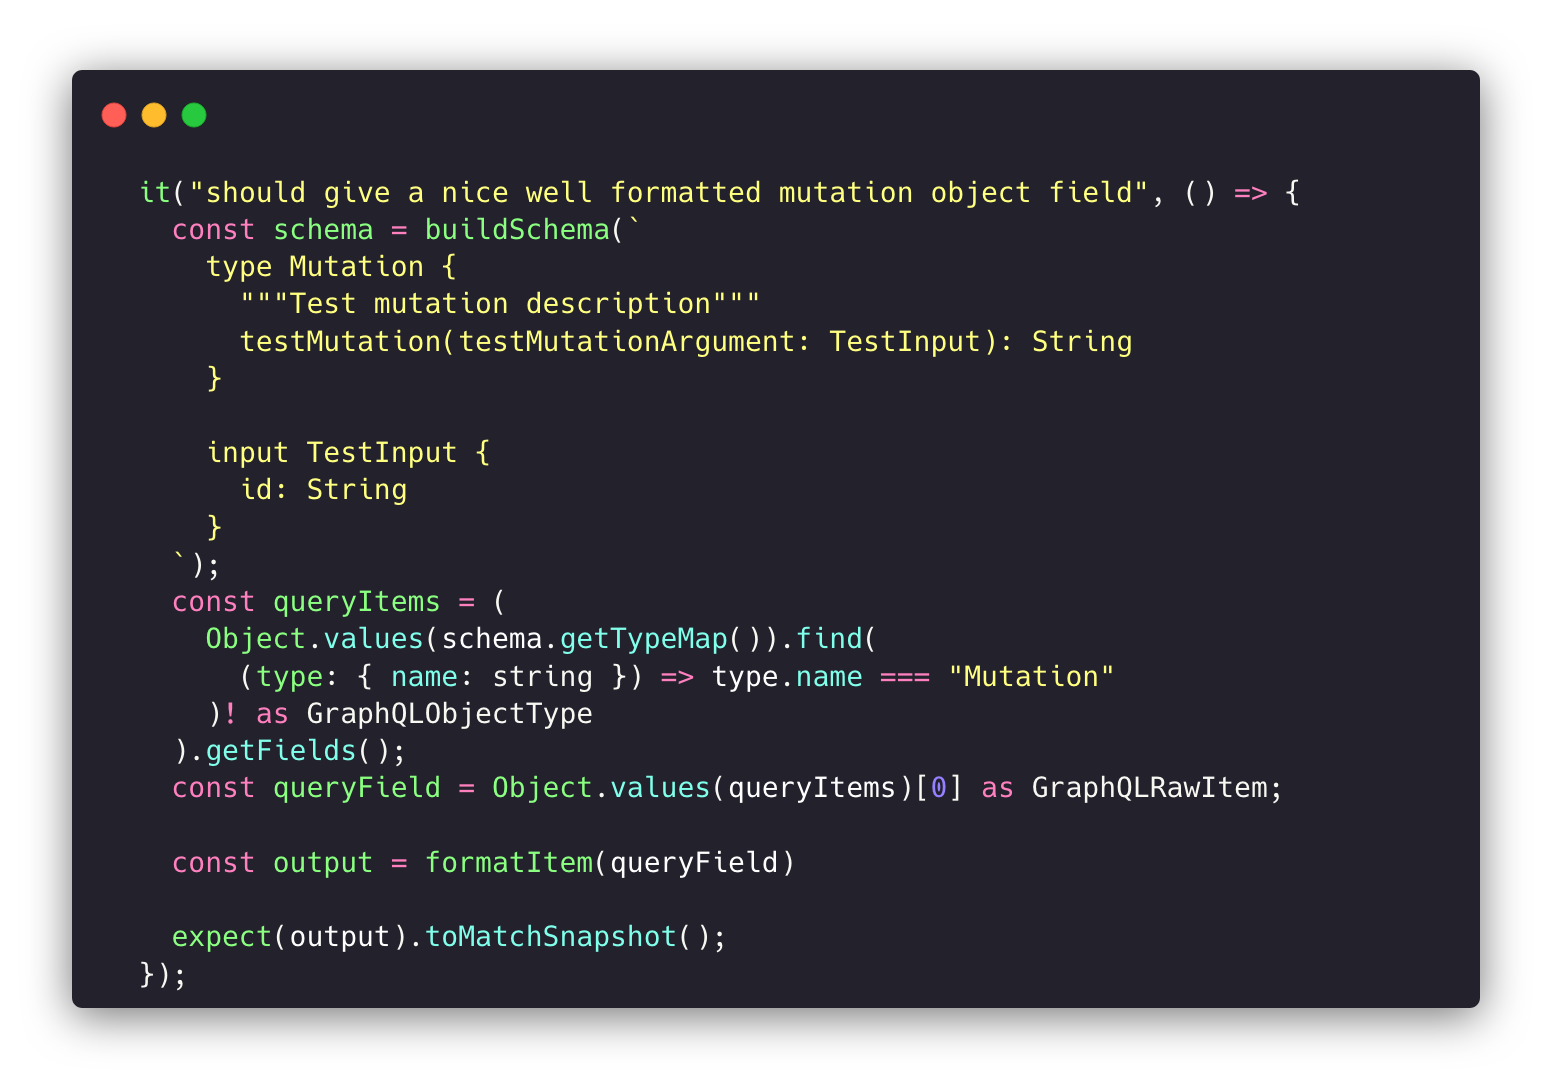
\includegraphics[width=0.6\textwidth]{figures/code/test1.png}
  \caption{Test formatItem Mutation Type}
  \label{f:test1}
\end{figure}

In the picture above, the mutation type is being tested. The will build a schema,
get the field from the AST and then format it.

\begin{figure}[H]
  \centering
  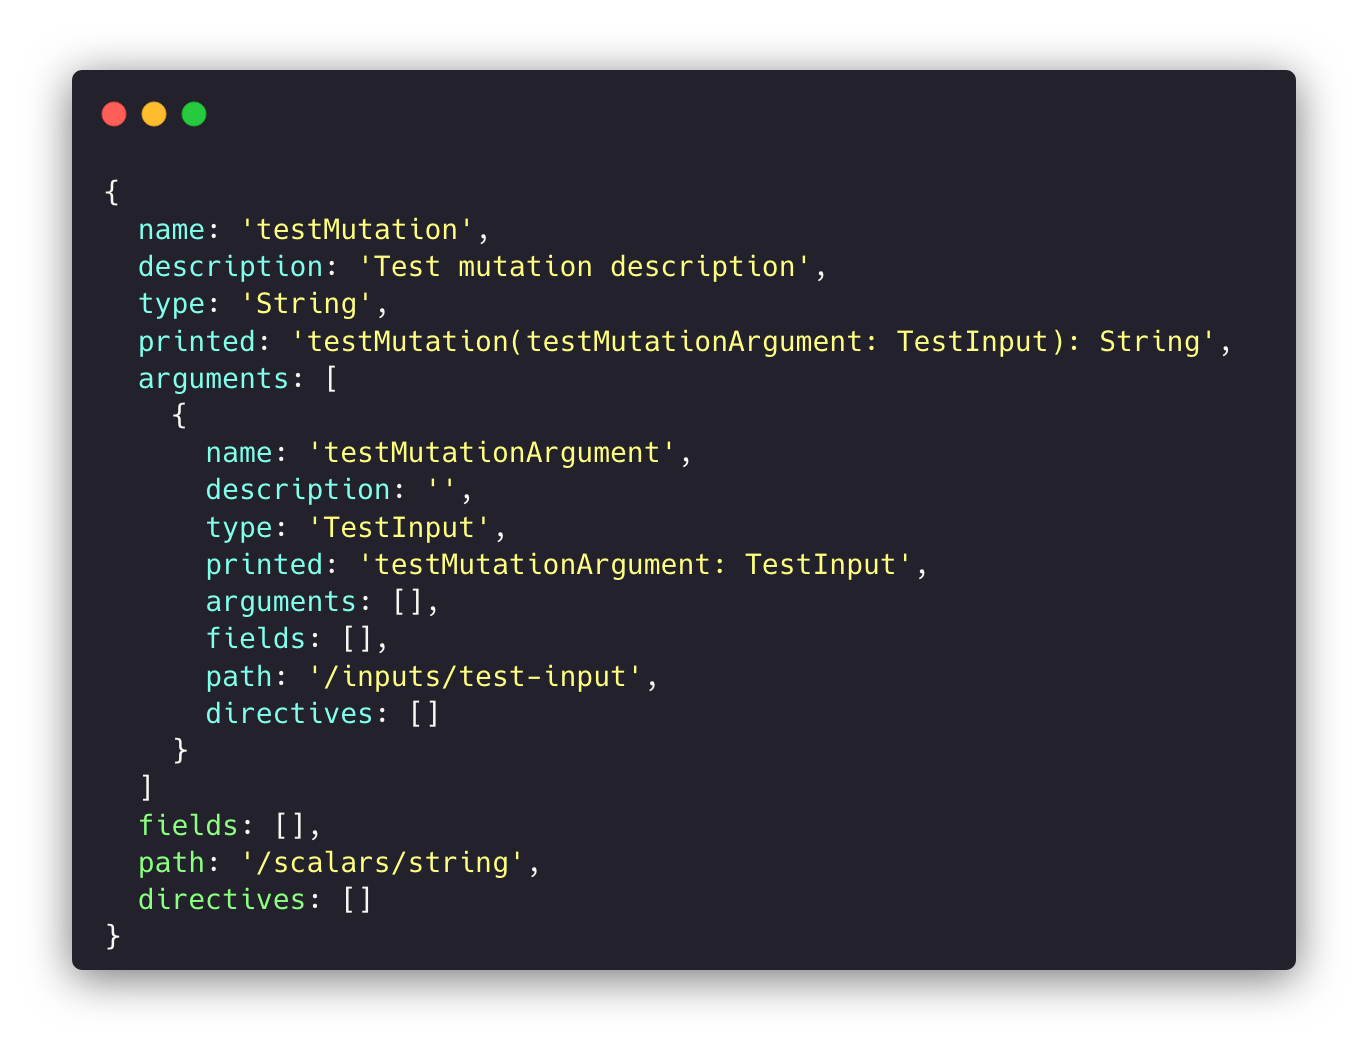
\includegraphics[width=0.6\textwidth]{figures/code/testMutation.png}
  \caption{Test Output}
  \label{f:testMutation}
\end{figure}

After that will then compare the formatted output with the snapshot, and if they
match, the test will pass. All the types are being tested and the screenshot
below shows the terminal output after \texttt{yarn test} which run all the tests
in the project.

\begin{figure}[H]
  \centering
  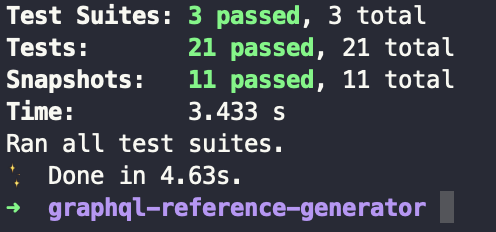
\includegraphics[width=0.6\textwidth]{figures/testspass.png}
  \caption{Passing Tests}
  \label{f:testspass}
\end{figure}

The output above confirms all passing tests, which is a good sign that the
functions used in the project are working as expected and covering multiple
uses-cases.
